\chapter{Background}
\label{chap:background}

This chapter introduces the contextual environment framework, evaluation concepts and benchmarks used throughout the thesis, and relates the simulation bottleneck to the reality gap.

\section{Contextual environments}
\label{sec:bg_cmdp}
% - CMDPs: fixed context and evolving state.
% - Levels are environment instances.
\textbf{Contextual MDPs.} We follow the framework established by \citet{kirk2023survey}, building on contextual Markov decision processes \citep{hallak2015contextual}. We consider the episodic setting, and model the environment as a Contextual-MDP (CMDP) $\mathcal{M} \triangleq ( \sS, \sA, \sO, \mathcal{T}, \Omega, R, \sC, P(\rc), \mathcal{P}_0, \gamma)$ with state, action and observation spaces $\sS$, $\sA$ and $\sO$ and discount factor $\gamma\in[0,1]$; $\mathscr{P}(\cdot)$ denotes probability distributions over the indicated space. In a CMDP, the reward function $R:\sS \times \sC \times \sA \rightarrow \sR$, observation kernel $\Omega: \sS \times \sC \rightarrow \mathscr{P}(\sO)$, transition kernel $\mathcal{T} : \sS \times \sC \times \sA \rightarrow \mathscr{P}(\sS)$, and initial state kernel $\mathcal{P}_0: \sC \rightarrow \mathscr{P}(\sS)$ can change with the \textit{context} $c\in\sC$, with $c \sim P(\rc)$ at the start of each episode. The CMDP is therefore a partially observable MDP with full state space $\sS \times \sC$. Each context $c$ maps one-to-one to a particular \textit{environment instance} $\mathcal{M}_c$, or \textit{level}, and thus represents the component of the state $(s,c)$ that cannot change during the episode, while $s$ evolves. We use \textit{level} and \textit{environment instance} interchangeably in Chapters~\ref{chap:deac} and~\ref{chap:dred}. The context need not be observable; the agent receives $o_t\sim\Omega(s_t,c)$ rather than the full state $(s_t,c)$. Deterministic observations are the special case in which $\Omega(s,c)$ is concentrated on a single observation.

\textbf{Policy.} The agent's policy $\pi$ selects actions from a distribution conditioned on the current observation or, for a recurrent policy, the observation history.

\section{The reality gap and the simulation bottleneck}
\label{sec:bg_sim2real}
% - Reality gap: discrepancies in interaction experience.
% - Zero-shot evaluation, performance gaps and sample efficiency.
% - Learned simulation and repeated engineering effort.
\textbf{The reality gap.} The \textit{reality gap} describes discrepancies between simulation and deployment conditions, historically studied by \citet{jakobi1995noise}. For an interaction protocol $u$ specifying scenario sampling, initialisation, action selection and horizon, let $\mathbb{P}_{\mathrm{sim}}^u$ and $\mathbb{P}_{\mathrm{target}}^u$ be the induced distributions over observable trajectories, including rewards where defined. Given a distance $d$ between these distributions, define
\begin{equation}\label{eq:bg_realitygap}
    \text{RealityGap}_d(u) \triangleq d(\mathbb{P}_{\mathrm{sim}}^u,\mathbb{P}_{\mathrm{target}}^u).
\end{equation}
The protocol and distance specify which aspects of environmental fidelity are assessed. For example, in Chapter~\ref{chap:persist}, the protocol replays the same action sequences in the learned simulator and the reference environment, comparing observation trajectories and omitting rewards. Choosing $d$ as the Fr\'echet Video Distance (FVD)~\citep{unterthiner2018towards} between the resulting video-clip distributions gives the reality-gap measure used to evaluate the world model.

\phantomsection\label{sec:bg_zsg}
\textbf{Zero-shot generalisation.} We evaluate a trained policy on previously unseen environment instances without further policy training on those instances \citep{darla,kirk2023survey}. Held-out contexts drawn from the same distribution test generalisation beyond the finite training set; contexts drawn from a different distribution additionally test robustness to distribution shift. In both cases, the policy's parameters remain fixed during evaluation.

\textbf{Performance gaps.} Following \citet{kirk2023survey}, we represent variation in environment conditions through context distributions. For a fixed policy $\pi$ and context distribution $p$, define
\begin{equation}\label{eq:bg_return}
    J_p(\pi) \triangleq \E_{c\sim p,\,\tau\sim(\pi,\mathcal{M}_c)}\!\left[\sum_{t=0}^{T-1}\gamma^t r_t\right],
\end{equation}
where $T$ is the episode horizon, $r_t$ the reward at time $t$, and $\tau$ a trajectory under $\pi$ in $\mathcal{M}_c$, including $s_0\sim\mathcal{P}_0(c)$. For context distributions $p$ and $q$, the performance gap is
% Retain the earlier equation keys as aliases for the shared definition.
\makeatletter
\begin{equation}\label{eq:bg_perfgap}
    \ltx@label{eq:bg_gengap}\ltx@label{eq:bg_sim2real}
    \text{PerfGap}(\pi;p,q) \triangleq J_p(\pi)-J_q(\pi).
\end{equation}
\makeatother
We assume the same task, comparable rewards, horizons and discounting, and evaluation without additional policy training. Table~\ref{tab:bg_gaps} gives particular comparisons.

\begin{table}[htbp]
\centering
\small
\caption{Performance gaps as choices of $p$ and $q$ in $\text{PerfGap}(\pi;p,q)$.}
\label{tab:bg_gaps}
\begin{tabularx}{\textwidth}{@{}>{\raggedright\arraybackslash}p{0.34\textwidth}>{\raggedright\arraybackslash}X>{\raggedright\arraybackslash}X@{}}
\toprule
\textbf{Quantity} & $p$ & $q$ \\
\midrule
$\text{Sim2RealGap}$ & $p_{\mathrm{sim}}$: simulated contexts & $p_{\mathrm{real}}$: real deployment contexts \\
\addlinespace
$\text{GenGap}$ (Chapters~\ref{chap:deac} and~\ref{chap:dred}) & $\widehat p_{\mathrm{train}}$: training set & $\widehat p_{\mathrm{test}}$: held-out set from the same distribution \\
\addlinespace
$\text{ShiftGap}$ (Chapter~\ref{chap:dred}) & $P_\Lambda$: adaptive or generated levels & $\widehat p_{\mathrm{train}}$: original training set \\
\bottomrule
\end{tabularx}
\end{table}

For $\text{GenGap}$, training and test instances are sampled independently from the same environment distribution. Their population trajectory laws therefore satisfy $\mathbb{P}_{\mathrm{train}}^u=\mathbb{P}_{\mathrm{test}}^u$, giving zero reality gap. The empirical context distributions $\widehat p_{\mathrm{train}}$ and $\widehat p_{\mathrm{test}}$ describe finite sets, whose returns can still differ. When the reality gap is closed, comparing training instances with held-out deployment instances becomes this generalisation problem.

In Chapter~\ref{chap:dred}, $P_\Lambda$ is an adaptive distribution over a buffer of existing or generated levels. Its $\text{ShiftGap}$ compares returns under this distribution with returns on the original training set.

\textbf{Sample efficiency.} Sample efficiency describes the amount of training interaction required to achieve a given level of performance. Performance may be measured on training instances or held-out instances; the latter also reflects generalisation.

\textbf{The simulation bottleneck.} The \textit{simulation bottleneck} concerns the repeated, domain-specific human engineering required to construct sufficiently faithful simulators and representative training scenarios. This burden seeks to reduce the reality gap and provide useful training experience. Figure~\ref{fig:intro_engineering_effort} illustrates approaches that shift parts of this work from manual specification to computation and data.\footnote{These examples are not exhaustive; the related-work sections of Chapters~\ref{chap:deac}--\ref{chap:persist} provide detailed literature reviews.}

With handcrafted simulators, domain randomisation varies simulated conditions to support transfer \citep{tobin2017domain}, while domain adaptation addresses discrepancies between simulation and deployment \citep{zhao2020simtoreal}. These methods reduce reliance on precisely matched conditions, but still require a simulator and a choice of training scenarios. An \textit{orchestrator} automates scenario selection or generation using, for example, a generative model or an LLM, corresponding to the second trend in the figure. RoboGen generates robotic tasks, scenes and training supervision \citep{wang2024robogen}; CUA-Gym generates computer-use tasks, environment states and verifiable rewards \citep{wang2026cuagym}. Such automation must supply both reliable and diverse environments \citep{li2026agentic}. DRED (Chapter~\ref{chap:dred}) learns the context distribution from example levels to generate new training instances.

Learning the simulator itself from data~\citep{hafner2025training,valevski2024diffusionmodelsrealtimegame,alonso2024diffusion} addresses the engineering of dynamics and observations, corresponding to the third trend. PERSIST (Chapter~\ref{chap:persist}) improves spatial memory and temporal coherence by maintaining an explicit 3D representation of the environment. Together, learning the context distribution and learning the simulator motivate approaches that scale with computation and data rather than human engineering effort.

\begin{figure}[htbp]
    \centering
    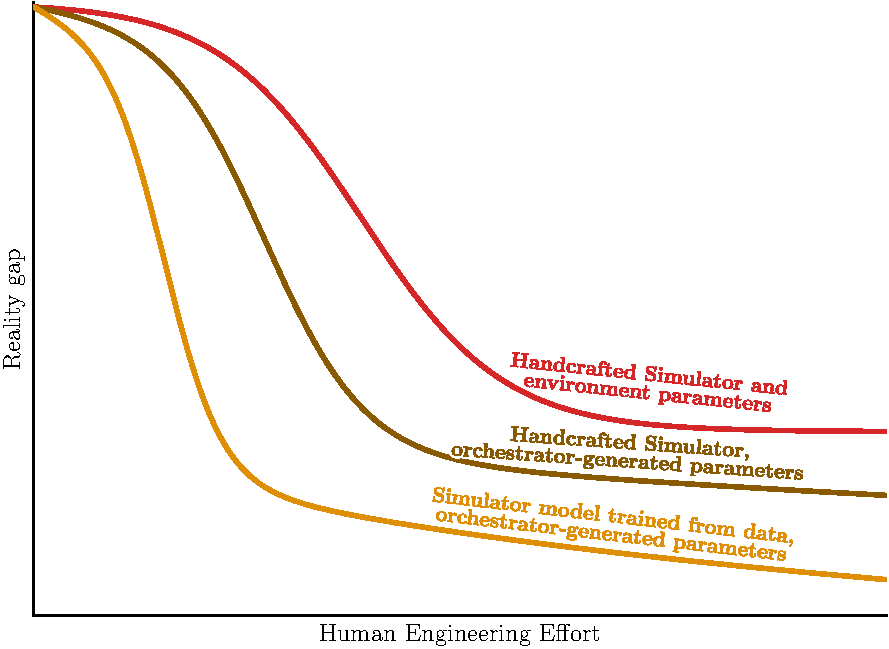
\includegraphics[width=\textwidth]{background/figures/engineering_effort.pdf}
    \caption[Conceptual engineering effort and reality gap.]{Automating scenario generation and learning simulators may reduce the human engineering needed to narrow the reality gap. The trends are conceptual, not measured performance--effort relationships or guaranteed rankings.}
    \label{fig:intro_engineering_effort}
\end{figure}

\section{Benchmarks and environments}
\label{sec:bg_environments}
% - Reproducible instances and controlled training-set size.
% - Benchmark properties and roles in the thesis.
The environments and benchmarks used to train and evaluate agents and world models in this thesis support a wide variety of configurable instances, each uniquely identified by a specified context. This enables reproducible instance selection, explicit control over the number of distinct instances available during training, and a clear separation between training and test sets. Together, they provide complementary settings for studying representation learning, environment generation and learned simulation.

\textbf{Procgen.} Procgen~\citep{procgen} is a suite of diverse discrete-control tasks with procedural levels selected by seed. Separate sets of training and held-out levels allow us to study instance overfitting and zero-shot generalisation.

\textbf{Brax/PixelBrax.} Brax and its pixel-based extension PixelBrax~\citep{brax2021github,mcinroe2025pixelbrax} provide continuous-control tasks with variation in initial conditions and video distractors. These environments extend our study of representation learning beyond Procgen to continuous control from pixels.

\textbf{Minigrid.} Minigrid~\citep{gym_minigrid} provides gridworld environments with explicitly parameterised layouts and objects. This control over level structure supports the generation of new instances and controlled studies of distribution shift.

\textbf{Procedural 3D worlds.} Minecraft-based environments, including MineDojo, and Luanti/Craftium~\citep{fan2022minedojo,luanti2024,malagon2025craftium} provide structured interactive worlds with spatial variation and persistent dynamics. World-generation seeds and scene parameters distinguish instances, making these environments suitable for learning and evaluating world models across diverse layouts and extended interactions.
